\documentclass[main]{subfiles}
\begin{document}
%@@@@@@@@@@@@@@@@@@@@@@@@@@@@@@
% summarizes lecture
% author: Doris Ling

\section{Bump Circuit}

% Doris

The Bump-Antibump circuit is comprised of a Differential Pair with the gates of the input transistors tied to the gates of two stacked transistors. 

\begin{figure}[htbp]
  \centering
  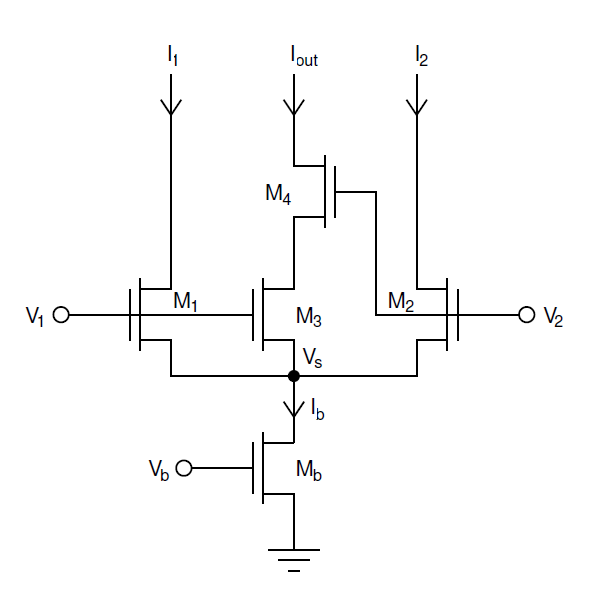
\includegraphics[scale=0.7]{pics/Bump-Antibump_circuit.png}
  \caption{Bump circuit}
  \label{fig:Bump-Antibump_circuit}
\end{figure}

If $V_1 >> V_2$ or $V_2 >> V_1$, then the circuit behaves as a Differential Pair with $I_{out}$ as a function of $V_2 -V_1$.

\begin{equation}
I_{out} = \frac{I_b}{1+\frac{4}{S}cosh^2 \frac{\kappa dV}{2U_T}} \geq 0
\end{equation}

where the transistor geometry factor, 

\begin{equation}
S = \frac{(W/L)_{middle}}{(W/L)_{outer}}
\end{equation}

If the difference between $V_1$ and $V_2$ is small, the stacked transistors will have similarly biased gates, and $I_{out}$ will reflect the sum of the two currents according to:

%shouldn't it be I_b-I_{out}???
\begin{equation}
I_1+I_2 = I_b+I_{out}= \frac{I_B}{1+ \frac{S}{4} cosh^{-2} \frac{\kappa dV}{2U_T}} \geq 0
\end{equation}

If the limit of $I_1$ + $I_2$ is taken as $\delta$ V $\rightarrow$ 0, the sum reaches an absolute minimum at 

\begin{equation}
I_1+I_{2_{min}} = \frac{I_b}{1+\frac{S}{4}} \geq 0
\end{equation}


\begin{figure}[htbp]
  \centering
  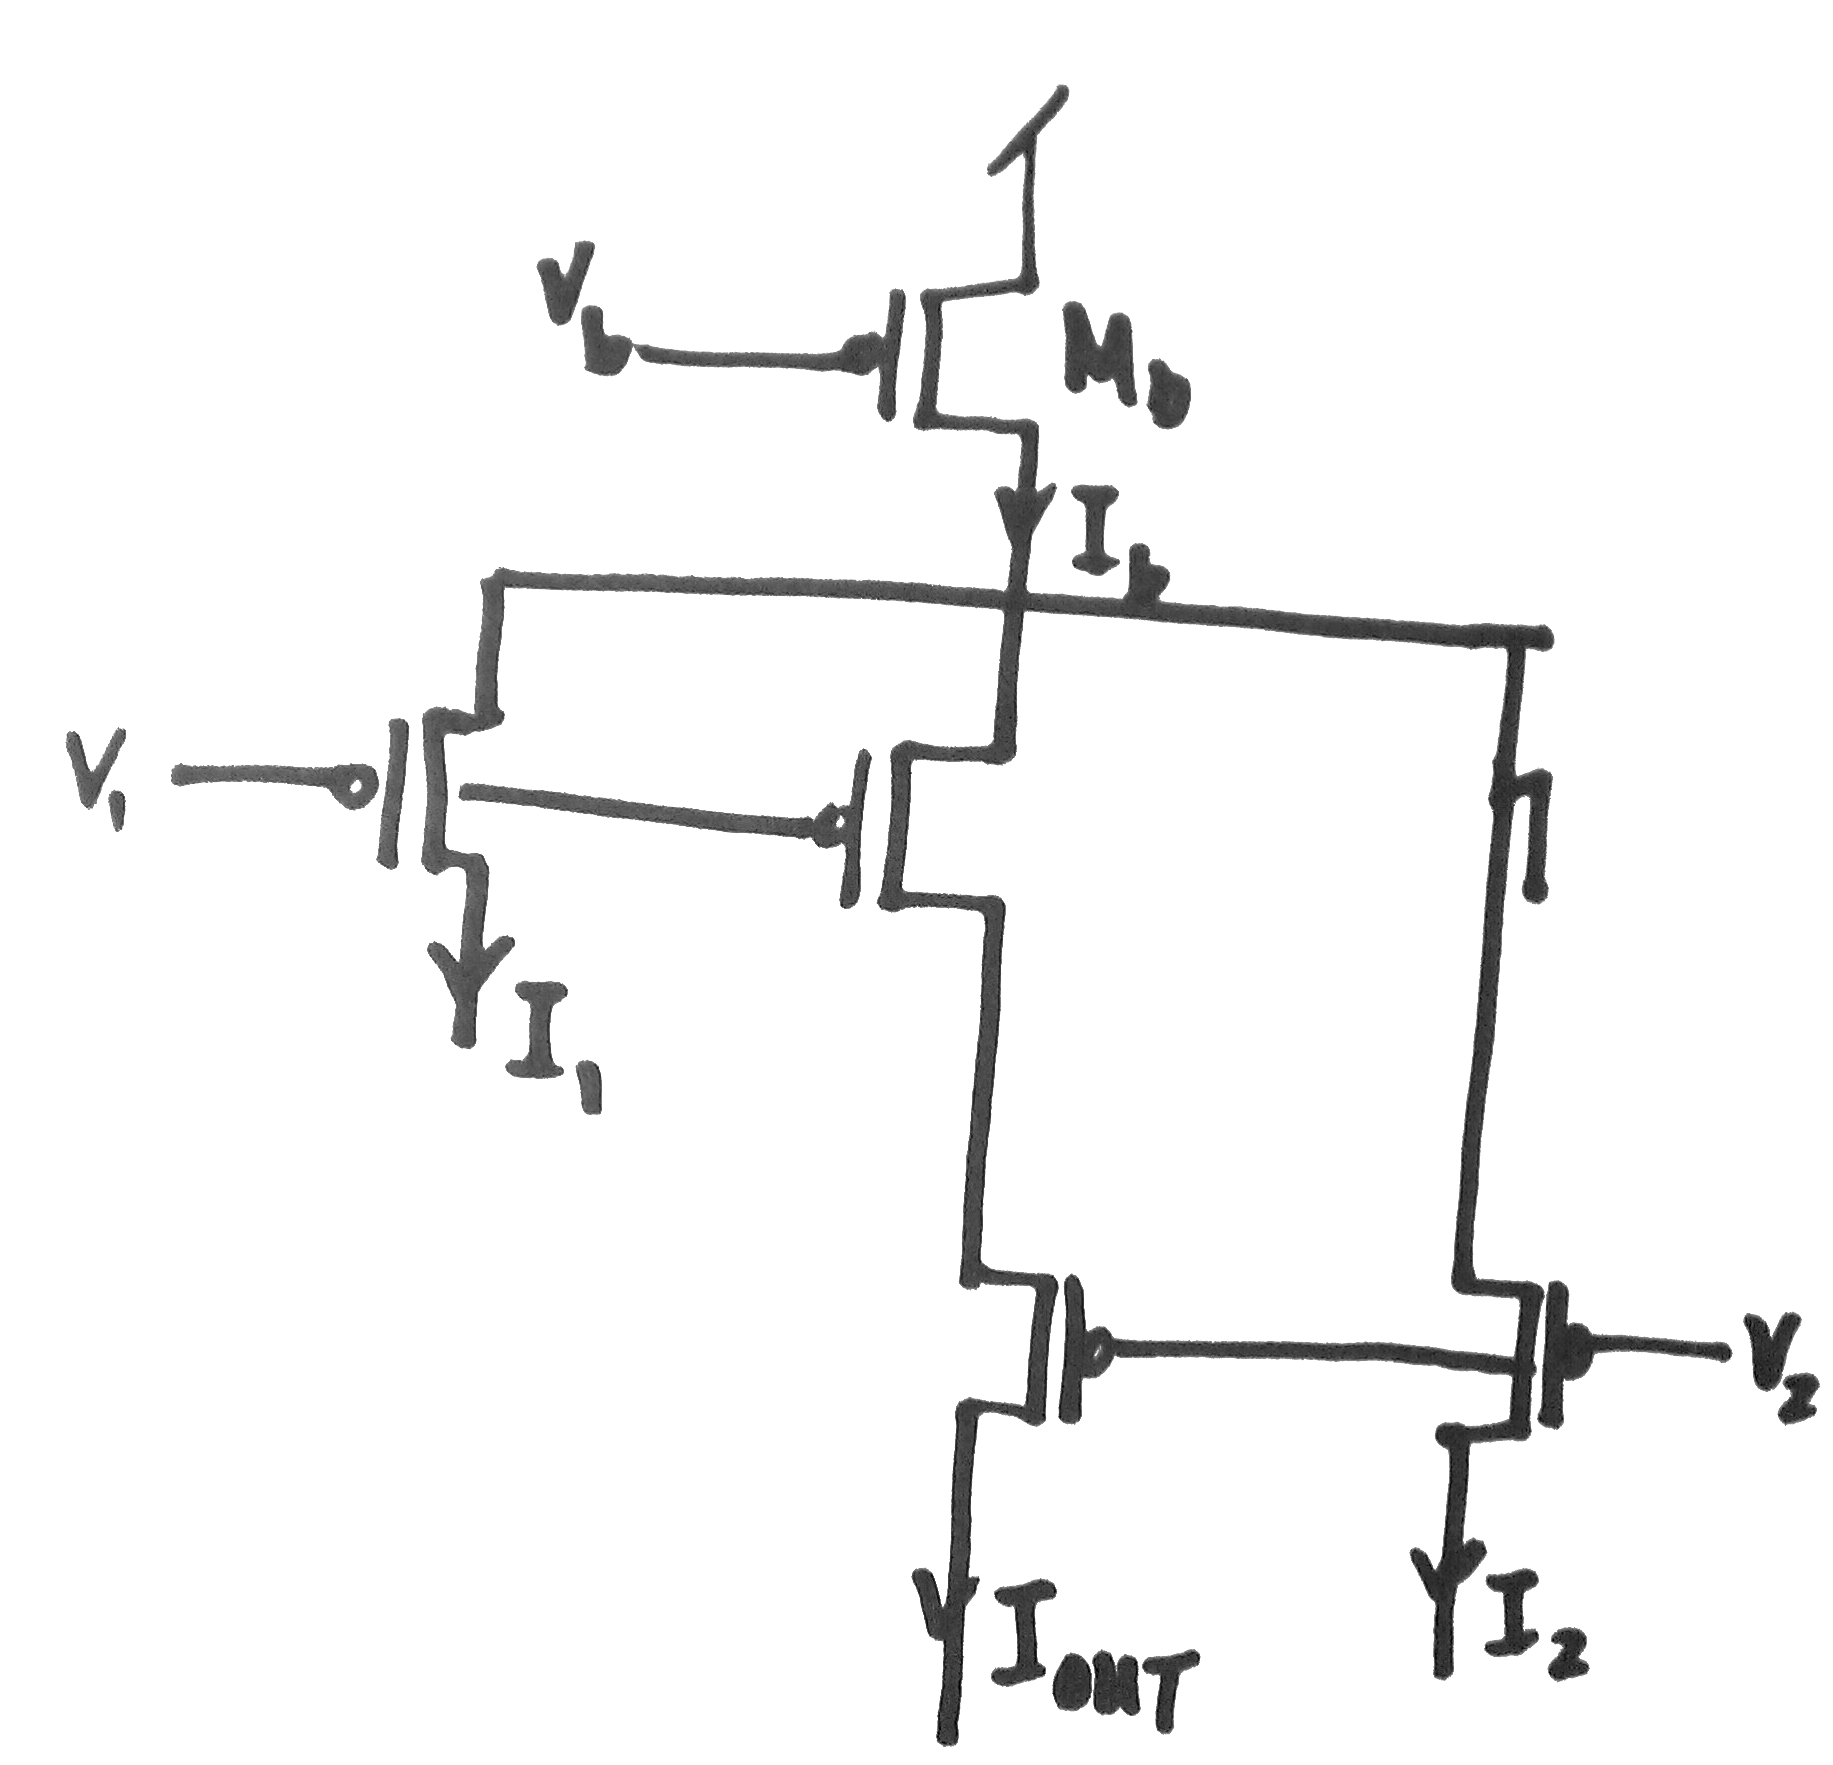
\includegraphics[scale=0.2]{pics/pFET_Bump_circuit}
  \caption{pFET Bump circuit}
  \label{fig:pFET_Bump_circuit}
\end{figure}
\end{document}